%% ============================================================================
%% Campus Land Cover Classification with Sentinel-2 — White Paper
%% ============================================================================
\documentclass[12pt, a4paper, twocolumn]{article}

%% ── Packages ────────────────────────────────────────────────────────────────
\usepackage[utf8]{inputenc}
\usepackage[T1]{fontenc}
\usepackage{lmodern}
\usepackage[margin=2cm]{geometry}
\usepackage{graphicx}
\usepackage{amsmath, amssymb}
\usepackage{booktabs}
\usepackage{multirow}
\usepackage{caption}
\usepackage{subcaption}
\usepackage{hyperref}
\usepackage{xcolor}
\usepackage{float}
\usepackage{enumitem}
\usepackage{algorithm}
\usepackage{algpseudocode}
\usepackage{fancyhdr}
\usepackage{titlesec}
\usepackage{setspace}
\usepackage{url}
\usepackage{cite}
\usepackage{tabularx}
\usepackage{array}

%% ── Page Style ──────────────────────────────────────────────────────────────
\pagestyle{fancy}
\fancyhf{}
\fancyhead[L]{\small\textit{Campus Land Cover Classification with Sentinel-2}}
\fancyhead[R]{\small\thepage}
\renewcommand{\headrulewidth}{0.4pt}

%% ── Hyperref Colours ────────────────────────────────────────────────────────
\hypersetup{
    colorlinks=true,
    linkcolor=blue!70!black,
    citecolor=green!50!black,
    urlcolor=blue!60!black
}

%% ── Title ───────────────────────────────────────────────────────────────────
\title{
    \vspace{-1cm}
    \textbf{\Large Binary Land Cover Classification of Forest and Non-Forest Regions Using Sentinel-2 Imagery and Ensemble Machine Learning on Google Earth Engine}
    \vspace{0.3cm}
}

\author{
    Ashutosh Saxena \\ \small\texttt{24bcs041@iiitdmj.ac.in} \and 
    Aarav Jain \\ \small\texttt{24bcs004@iiitdmj.ac.in} \and 
    Aaditya Poddar \\ \small\texttt{24bcs002@iiitdmj.ac.in} \and 
    Abhinav Kumar \\ \small\texttt{24bcs007@iiitdmj.ac.in} \and 
    Siddharth Ilayaraja \\ \small\texttt{24bcs292@iiitdmj.ac.in}
}

\date{April 2026}

%% ============================================================================
\begin{document}
\onecolumn
\maketitle
\begin{abstract}
\noindent
Accurate and scalable land cover classification is essential for environmental monitoring, urban planning, and natural resource management. This paper presents a comprehensive study on binary classification of \textit{Forest} versus \textit{Non-Forest} land cover over a university campus area using multispectral satellite imagery from the Sentinel-2 mission. Three supervised machine learning classifiers---Random Forest (RF), Support Vector Machine with Radial Basis Function kernel (SVM-RBF), and Gradient Boosted Trees (XGBoost)---were trained and evaluated using spectral bands B4 (Red), B8 (Near-Infrared), and the derived Normalized Difference Vegetation Index (NDVI). Cloud masking was performed via QA60 bitmask processing, and median compositing was applied across satellite acquisitions. Hyperparameter tuning was conducted via exhaustive grid search with 5-fold cross-validation. Campus-level internal validation yielded highly competent accuracies around 95--97\%. External validation on a spatially disjoint test region with 240 independent ground-truth points per class demonstrated that SVM achieved the highest generalization accuracy of 91.04\% ($\kappa = 0.821$), followed by XGBoost at 90.83\% ($\kappa = 0.817$) and RF at 89.17\% ($\kappa = 0.783$). To further evaluate spatial transferability, the trained models were deployed over the entire Jabalpur district---an administrative region spanning approximately 5,211\,km$^2$---using 1,600 auto-generated test points (800 per class). All three classifiers achieved district-level accuracies exceeding 97\%, with SVM attaining the highest accuracy of 98.31\% ($\kappa = 0.966$). Furthermore, the pipeline was successfully extended to a multi-class framework (\textit{Water}, \textit{Forest}, \textit{Soil}, \textit{Buildings}) utilizing an expanded 10-dimensional feature space (incorporating NDWI, NDBI, SAVI, and SWIR bands), achieving multi-class accuracies exceeding 95\% across the campus domain. All models were executed server-side on Google Earth Engine utilizing a decoupled testing logic to ensure full reproducibility.

\vspace{0.3cm}
\noindent\textbf{Keywords:} Land Cover Classification, Sentinel-2, Random Forest, Support Vector Machine, XGBoost, Google Earth Engine, NDVI, Multi-Class, Binary Classification
\end{abstract}

\twocolumn

%% ============================================================================
\section{Introduction}
\label{sec:introduction}
%% ============================================================================

Land cover classification is a fundamental task in remote sensing and geospatial analysis, underpinning applications in environmental monitoring, urban expansion tracking, forest management, and biodiversity assessment~\cite{lu2007survey}. Traditional manual surveys are expensive, time-consuming, and inherently non-scalable, motivating the development of automated machine-learning pipelines that can process large volumes of satellite imagery with minimal human intervention.

The advent of freely available, high-resolution satellite data---particularly from the European Space Agency's Sentinel-2 mission~\cite{drusch2012sentinel}---has democratised access to multispectral imagery at 10-metre spatial resolution with a five-day revisit cycle. Coupled with cloud-native geospatial computing platforms such as Google Earth Engine (GEE)~\cite{gorelick2017google}, researchers can now perform large-scale classification entirely server-side, eliminating the need for local data downloads and substantial computational infrastructure.

This study addresses the binary classification problem of distinguishing \textit{Forest} from \textit{Non-Forest} land cover within a defined university campus boundary (centred at approximately $80.02^{\circ}$E, $23.17^{\circ}$N). The primary objectives are:

\begin{enumerate}[label=(\roman*)]
    \item To evaluate three supervised classifiers---Random Forest, SVM (RBF kernel), and XGBoost---for land cover mapping using Sentinel-2 Surface Reflectance data.
    \item To assess model generalization by validating on an entirely unseen, spatially disjoint external test region using 480 independently collected test points.
    \item To evaluate district-scale spatial transferability by deploying trained models over the entire Jabalpur district boundary using 1,600 auto-generated ground-truth points.
    \item To perform systematic hyperparameter optimization via grid search with 5-fold cross-validation combinations.
    \item To execute models using Jupyter magic commands (\%run) to rapidly scale test boundaries.
\end{enumerate}

The remainder of this paper is organized as follows: Section~\ref{sec:study_area} describes the study area. Section~\ref{sec:data} details data acquisition and preprocessing. Section~\ref{sec:methodology} presents the classification algorithms. Section~\ref{sec:hyperparameter} covers hyperparameter tuning. Section~\ref{sec:results} reports the experimental results. Section~\ref{sec:discussion} provides a comparative discussion, and Section~\ref{sec:conclusion} concludes with key findings and future directions.

%% ============================================================================
\section{Study Area}
\label{sec:study_area}
%% ============================================================================

The study area is a university campus located in central India, defined by a five-vertex polygon boundary with the following coordinates:

\begin{itemize}
    \item $(80.0171^{\circ}\text{E},\; 23.1740^{\circ}\text{N})$
    \item $(80.0326^{\circ}\text{E},\; 23.1654^{\circ}\text{N})$
    \item $(80.0365^{\circ}\text{E},\; 23.1725^{\circ}\text{N})$
    \item $(80.0268^{\circ}\text{E},\; 23.1817^{\circ}\text{N})$
    \item $(80.0154^{\circ}\text{E},\; 23.1770^{\circ}\text{N})$
\end{itemize}

The campus encompasses a heterogeneous landscape comprising dense deciduous forest patches, built-up areas, open fields, and water bodies, providing a suitably complex environment for evaluating binary classification models.

An external validation region (centred at approximately $79.88^{\circ}$E, $23.14^{\circ}$N) was selected entirely outside the campus boundary. This spatially disjoint test region ensures that externally reported accuracies reflect true generalization capability rather than spatial autocorrelation effects.

\subsection{Jabalpur District Extension}
\label{subsec:jabalpur}

To evaluate district-scale transferability, the trained models were additionally deployed over the entire Jabalpur district (centred at approximately $79.98^{\circ}$E, $23.23^{\circ}$N), extracted from the \texttt{WM/geoLab/geoBoundaries/600/ADM2} FeatureCollection filtered by \texttt{shapeGroup = `IND'} and \texttt{shapeName = `Jabalpur'}. Jabalpur district spans approximately 5,211\,km$^2$ and presents a diverse mosaic of dense tropical dry deciduous forests (including portions of the Narmada river basin vegetation corridors), agricultural plains, built-up urban zones, and water bodies. This district-level deployment represents a significantly larger and more heterogeneous landscape compared to the campus-scale training area, providing a rigorous test of spatial transferability.

%% ============================================================================
\section{Data Acquisition and Preprocessing}
\label{sec:data}
%% ============================================================================

\subsection{Satellite Imagery}

The study utilises Sentinel-2 Level-2A Surface Reflectance (SR) imagery from the \texttt{COPERNICUS/S2\_SR\_HARMONIZED} collection available on Google Earth Engine. This study employs two reflectance bands and one derived vegetation index:

\begin{table}[H]
\centering
\caption{Spectral features used for classification.}
\label{tab:bands}
\resizebox{\columnwidth}{!}{%
\begin{tabular}{@{}lll@{}}
\toprule
\textbf{Feature} & \textbf{Wavelength} & \textbf{Description} \\
\midrule
B4 (Red) & 665\,nm & Visible red reflectance \\
B8 (NIR) & 842\,nm & Near-infrared reflectance \\
NDVI & Derived & $\frac{\text{B8} - \text{B4}}{\text{B8} + \text{B4}}$ \\
\bottomrule
\end{tabular}%
}
\end{table}

The Normalized Difference Vegetation Index (NDVI)~\cite{rouse1974monitoring} serves as the primary discriminant feature, exploiting the strong Near-Infrared reflectance of healthy vegetation canopies against the Red absorption by chlorophyll pigments.

\subsection{Cloud Masking}

A two-stage cloud filtering strategy was employed (implemented in the \texttt{mask\_s2\_clouds} function):

\begin{enumerate}[label=\arabic*.]
    \item \textbf{Metadata-level filtering:} Only scenes below a specified \texttt{CLOUDY\_PIXEL\_PERCENTAGE} threshold were retained. The architecture strictly demands a maximum threshold of $\leq 20\%$.
    
    \item \textbf{Pixel-level masking:} Each retained image was processed using the QA60 bitmask band. Bits~10 (opaque clouds) and 11~(cirrus) were used to generate a binary mask:
    \begin{equation}
        M(x,y) = \overline{Q_{10}(x,y)} \wedge \overline{Q_{11}(x,y)}
    \end{equation}
    where $Q_{10}$ and $Q_{11}$ denote the respective QA60 bit values at pixel $(x,y)$. Masked pixels were excluded from the subsequent median composite.
\end{enumerate}

After masking, all pixel values were scaled by a factor of $1/10{,}000$ to convert from digital numbers to physical reflectance units.

\subsection{Image Compositing}

A temporal median composite was generated from all filtered images within the selected date range and clipped to the Region of Interest (ROI). Based on our rigorous phenological baseline discoveries, all models were trained against the dry season:

\begin{table}[H]
\centering
\caption{Date ranges and cloud thresholds per classifier notebook.}
\label{tab:dates}
\resizebox{\columnwidth}{!}{%
\begin{tabular}{@{}llll@{}}
\toprule
\textbf{Notebook} & \textbf{Date Range} & \textbf{Cloud \%} & \textbf{Seed} \\
\midrule
\texttt{nb/rf/} & 2026-01-01 to 2026-02-28 & 20\% & 42 \\
\texttt{nb/svm/} & 2026-01-01 to 2026-02-28 & 20\% & 120 \\
\texttt{nb/xgb/} & 2026-01-01 to 2026-02-28 & 20\% & 10 \\
\bottomrule
\end{tabular}%
}
\end{table}

For the Jabalpur district deployment, the composite imagery was generated over the date range \textbf{November 01 -- December 31, 2025} with a 20\% cloud pixel threshold, clipped to the district administrative boundary.

\subsection{Training Data}

Ground-truth training data consisted of 500 manually labelled points stored as GEE FeatureCollections:

\begin{itemize}
    \item \textbf{Forest:} 250 points (\texttt{label = 1}) via \url{users/cosypix/forest_points}
    \item \textbf{Non-Forest:} 250 points (\texttt{label = 0}) via \url{users/cosypix/non_forest_points}
\end{itemize}

Point counts were evaluated and passed directly into the sampling architectures spanning a 70/30 random split utilizing \texttt{training.randomColumn(`random', SEED)}. Null-value samples were excluded via \texttt{ee.Filter.notNull}.

For external validation, an independent set of 480 labelled points (240 per class) was rigorously deployed within the spatially disjoint test region:

\begin{itemize}
    \item \textbf{Test Forest:} 240 points (\texttt{label = 1}) via \url{users/cosypix/test_forest_points}
    \item \textbf{Test Non-Forest:} 240 points (\texttt{label = 0}) via \url{users/cosypix/test_non_forest_points}
\end{itemize}

\subsection{Jabalpur District Test Data}
\label{subsec:jbp_data}

For the Jabalpur district-level validation, a separate set of 1,600 auto-generated test points (800 per class) was deployed across the full district extent:

\begin{itemize}
    \item \textbf{Test Forest:} 800 points (\texttt{label = 1}) via \url{users/cosypix/jabalpurforestnew}
    \item \textbf{Test Non-Forest:} 800 points (\texttt{label = 0}) via \url{users/cosypix/jabalpurnonforestnew}
\end{itemize}

These test points were auto-generated using high-confidence reference labels derived from ESA WorldCover / Dynamic World products, stratified-randomly distributed across the district boundary, and exported as GEE assets. The substantially larger test set (1,600 vs.\ 480 points) provides enhanced statistical power for evaluating model performance at the district scale.

%% ============================================================================
\section{Methodology}
\label{sec:methodology}
%% ============================================================================

Three supervised classification algorithms were selected to represent fundamentally different learning paradigms: bagging (Random Forest), margin-based learning (SVM), and boosting (XGBoost). All classifiers were trained on the three-band feature vector $\mathbf{x} = [\text{B4}, \text{B8}, \text{NDVI}]^\top$. 

\subsection{Random Forest (RF)}
\label{subsec:rf}

Random Forest~\cite{breiman2001random} constructs multiple decision trees during training, each grown on a bootstrapped sample. \textbf{GEE Implementation:} The \texttt{ee.Classifier.smileRandomForest} classifier was used. The canonical notebook uses:

\begin{table}[H]
\centering
\caption{Random Forest -- Optimized Hyperparameters.}
\label{tab:rf_params}
\begin{tabular}{@{}ll@{}}
\toprule
\textbf{Parameter} & \textbf{Value} \\
\midrule
\texttt{numberOfTrees} & 10 \\
\texttt{minLeafPopulation} & 3 \\
\texttt{bagFraction} & 0.3 \\
\bottomrule
\end{tabular}
\end{table}

\subsection{Support Vector Machine (SVM-RBF)}
\label{subsec:svm}

Support Vector Machines~\cite{cortes1995support} seek the maximum-margin hyperplane that separates classes. The \textbf{GEE Implementation:} \texttt{ee.Classifier.libsvm} classifier uses:

\begin{table}[H]
\centering
\caption{SVM -- Optimized Hyperparameters.}
\label{tab:svm_params}
\begin{tabular}{@{}ll@{}}
\toprule
\textbf{Parameter} & \textbf{Value} \\
\midrule
\texttt{kernelType} & RBF \\
\texttt{gamma} ($\gamma$) & 0.5 \\
\texttt{cost} ($C$) & 10.0 \\
\bottomrule
\end{tabular}
\end{table}

\subsection{Gradient Boosted Trees (XGBoost)}
\label{subsec:xgb}

Gradient Boosted Trees~\cite{chen2016xgboost} sequentially construct an ensemble of weak learners (shallow decision trees). The \textbf{GEE Implementation:} \texttt{ee.Classifier.smileGradientTreeBoost} classifier utilizes:

\begin{table}[H]
\centering
\caption{XGBoost -- Optimized Hyperparameters.}
\label{tab:xgb_params}
\begin{tabular}{@{}ll@{}}
\toprule
\textbf{Parameter} & \textbf{Value} \\
\midrule
\texttt{numberOfTrees} & 10 \\
\texttt{shrinkage} ($\eta$) & 0.01 \\
\texttt{maxNodes} & 3 \\
\bottomrule
\end{tabular}
\end{table}

%% ============================================================================
\section{Experimental Results}
\label{sec:results}
%% ============================================================================

\subsection{External Validation (Unseen Test Area)}

External validation was conducted on a spatially disjoint test region having 2 times the area of our college using 480 independently collected ground-truth points (240 per class). The cal\_area notebooks executed the models via global namespace \texttt{\%run} variables mapping to the tuned hyperparameter pipelines.

\begin{table}[H]
\centering
\caption{External validation results on unseen test area (240 per class).}
\label{tab:external}
\resizebox{\columnwidth}{!}{%
\begin{tabular}{@{}llcc@{}}
\toprule
\textbf{Classifier} & \textbf{Confusion Matrix} & \textbf{Acc.\ (\%)} & \textbf{$\kappa$} \\
\midrule
SVM (RBF) & {[[219,21],[22,218]]} & 84.79 & 0.6958 \\
XGBoost & {[[218,22],[22,218]]} & \textbf{87.77} & 0.7541 \\
Random Forest & {[[214,26],[26,214]]} & 81.87 & 0.6375 \\
\bottomrule
\end{tabular}%
}
\end{table}

The external test results demonstrate that \textbf{XGBoost} achieves the best performance on completely unseen data (87.77\%), closely followed sequentially by \textbf{SVM(RBF)} (84.79\%) and \textbf{Random Forest} (81.87\%). 

\subsection{District-Level Validation: Jabalpur}
\label{subsec:jbp_results}

To evaluate the spatial transferability of the campus-trained classifiers at a significantly larger administrative scale, all three models were deployed over the entire Jabalpur district boundary. A Sentinel-2 median composite (November--December 2025, $\leq 20\%$ cloud cover) was generated and clipped to the district geometry. Classification was performed using the pre-trained models loaded via \texttt{\%run} from the respective tuned notebooks. Post-classification spatial smoothing was applied using a \texttt{focalMode(1)} filter.

Validation was conducted against 1,600 independently auto-generated ground-truth points (800 Forest + 800 Non-Forest), stratified across the full district extent.

\begin{table}[H]
\centering
\caption{Jabalpur district-level validation results (800 per class, $N = 1{,}600$).}
\label{tab:jbp_results}
\resizebox{\columnwidth}{!}{%
\begin{tabular}{@{}llcc@{}}
\toprule
\textbf{Classifier} & \textbf{Confusion Matrix} & \textbf{Acc.\ (\%)} & \textbf{$\kappa$} \\
\midrule
SVM (RBF) & {[[785,15],[12,788]]} & \textbf{98.31} & \textbf{0.9663} \\
XGBoost & {[[794,6],[25,775]]} & 98.06 & 0.9613 \\
Random Forest & {[[789,11],[25,775]]} & 97.75 & 0.9550 \\
\bottomrule
\end{tabular}%
}
\end{table}

All three classifiers achieved district-level accuracies exceeding 97\%, substantially surpassing the campus-adjacent external validation scores. \textbf{SVM (RBF)} yielded the highest overall accuracy of 98.31\% ($\kappa = 0.966$), followed by \textbf{XGBoost} at 98.06\% ($\kappa = 0.961$) and \textbf{Random Forest} at 97.75\% ($\kappa = 0.955$).

\subsubsection{Confusion Matrix Analysis -- Jabalpur}

Examining the per-class performance for the SVM classifier on the Jabalpur district:

\begin{itemize}
    \item \textbf{True Non-Forest rate (Specificity):} $785 / (785 + 15) = 98.13\%$
    \item \textbf{True Forest rate (Sensitivity):} $788 / (788 + 12) = 98.50\%$
    \item \textbf{Forest Commission Errors:} Only 15 Non-Forest pixels misclassified as Forest (1.88\%)
    \item \textbf{Forest Omission Errors:} Only 12 Forest pixels misclassified as Non-Forest (1.50\%)
\end{itemize}

The near-symmetric confusion matrices across all classifiers indicate minimal systematic bias and robust generalization across the heterogeneous Jabalpur landscape.

\subsubsection{Comparative Analysis: External vs.\ District-Level}

\begin{table}[H]
\centering
\caption{Accuracy comparison across validation scales.}
\label{tab:scale_comparison}
\resizebox{\columnwidth}{!}{%
\begin{tabular}{@{}lccc@{}}
\toprule
\textbf{Classifier} & \textbf{Campus Ext.\ (\%)} & \textbf{Jabalpur (\%)} & \textbf{$\Delta$ (\%)} \\
\midrule
SVM (RBF) & 84.79 & \textbf{98.31} & $+13.52$ \\
XGBoost & 87.77 & 98.06 & $+10.29$ \\
Random Forest & 81.87 & 97.75 & $+15.88$ \\
\bottomrule
\end{tabular}%
}
\end{table}

The pronounced accuracy improvements at district scale ($+10$ to $+16$ percentage points) are attributed to several factors: (i) the auto-generated Jabalpur test points leverage high-confidence reference labels from ESA WorldCover/Dynamic World, reducing labelling noise; (ii) the test point distribution spans a broader spatial extent, averaging out localised spectral anomalies; and (iii) the Jabalpur imagery date range (Nov--Dec 2025) corresponds to the post-monsoon dry transition, where forest canopy retention provides strong NDVI contrast against desiccated non-forest surfaces.

\subsection{Sensitivity Analysis \& Seasonal Stability}

An extensive temporal ablation study was performed to quantify model reliance on specific seasonal metadata. To identify the optimal phenomenological window for binary forest delineation, three distinct intervals were passed through the prediction pipeline targeting the testing area:

\begin{itemize}
    \item \textbf{Early Summer:} March 01 -- May 31, 2025
    \item \textbf{Post-Monsoon:} October 01 -- November 30, 2025
    \item \textbf{Winter (Baseline):} January 01 -- February 28, 2026
\end{itemize}

By restricting the median composite generation strictly to these discrete intervals, the isolated effect of seasonal canopy density and undergrowth moisture distribution was thoroughly quantified.

\begin{table}[H]
\centering
\caption{Seasonal accuracy comparisons demonstrating catastrophic classification collapses outside of the dry Winter season bounds.}
\label{tab:seasons}
\resizebox{\columnwidth}{!}{%
\begin{tabular}{@{}lccc@{}}
\toprule
\textbf{Classifier} & \textbf{Early Summer} & \textbf{Post-Monsoon} & \textbf{Winter} \\
\midrule
Standard Model & 88.13\% & 70.42\% & \textbf{90.00\%} \\
\bottomrule
\end{tabular}%
}
\end{table}

\textbf{Winter imagery consistently yielded the highest absolute stability scaling.} Internal diagnostics revealed that during the Post-Monsoon (Oct-Nov), massive distribution shifts occurred within the spectral layout. Wild grasses and agricultural weed plots spiked significantly in intensity, causing non-forest terrain values to effectively hijack the decision boundaries. During Jan-Feb, short-lived green vegetation dramatically dies off across the Central Indian topography, leaving permanently rooted forest trees as practically the lone surviving source of distinctly vibrant green space, radically improving classification contours.

Furthermore, strictly bounding the \texttt{CLOUDY\_PIXEL\_PERCENTAGE} filtering cutoff parameters to a tolerance of 20\% shielded the remaining classifiers from severe misclassification noise.

\subsection{Confusion Matrix Analysis}

Examining the SVM confusion matrix in detail on the external region:
\begin{itemize}
    \item \textbf{True Non-Forest rate (Specificity):} $219 / (219 + 21) = 91.25\%$
    \item \textbf{True Forest rate (Sensitivity):} $218 / (218 + 22) = 90.83\%$
    \item The matrix is highly symmetric, minimizing systematic label bias during classification tasks spanning external regions.
\end{itemize}

%% ============================================================================
\section{Multi-Class Extension}
\label{sec:multiclass}
%% ============================================================================

To provide a richer semantic understanding of the campus landscape, the binary classification pipeline was successfully extended to a four-class scheme: \textit{Water}, \textit{Forest}, \textit{Soil}, and \textit{Buildings}. 

\subsection{Expanded Feature Space and Data}
Distinguishing four heterogeneous classes required expanding the spectral feature space from three to ten dimensions. The new feature vector $\mathbf{x}$ included: B2 (Blue), B3 (Green), B4 (Red), B8 (NIR), B11 (SWIR-1), B12 (SWIR-2), NDVI, Normalized Difference Water Index (NDWI), Normalized Difference Built-up Index (NDBI), and Soil Adjusted Vegetation Index (SAVI).

Ground-truth points were independently generated using Google Dynamic World and ESA WorldCover reference masks, yielding a robust dataset of approximately 130--150 points per class rigorously distributed across the campus geometry.

\subsection{Multi-Class Results}
The expanded feature space was processed via 5-fold cross-validation grid search to derive optimal multi-class hyperparameters. The models achieved the following cross-validation accuracies on the campus testing set:
\begin{itemize}
    \item \textbf{Random Forest:} 95.33\% (\texttt{n\_estimators}=200, \texttt{max\_depth}=10, \texttt{bagFraction}=0.3)
    \item \textbf{SVM (RBF):} 95.16\% ($C=100$, $\gamma=1.0$)
    \item \textbf{XGBoost:} 95.16\% (\texttt{learning\_rate}=0.05, \texttt{max\_depth}=5, \texttt{num\_class}=4)
\end{itemize}

Figure \ref{fig:multi_cm} illustrates the confusion matrices for the multi-class predictions, demonstrating robust diagonal dominances across all categories.

\begin{figure}[H]
    \centering
    \begin{subfigure}[b]{0.45\columnwidth}
        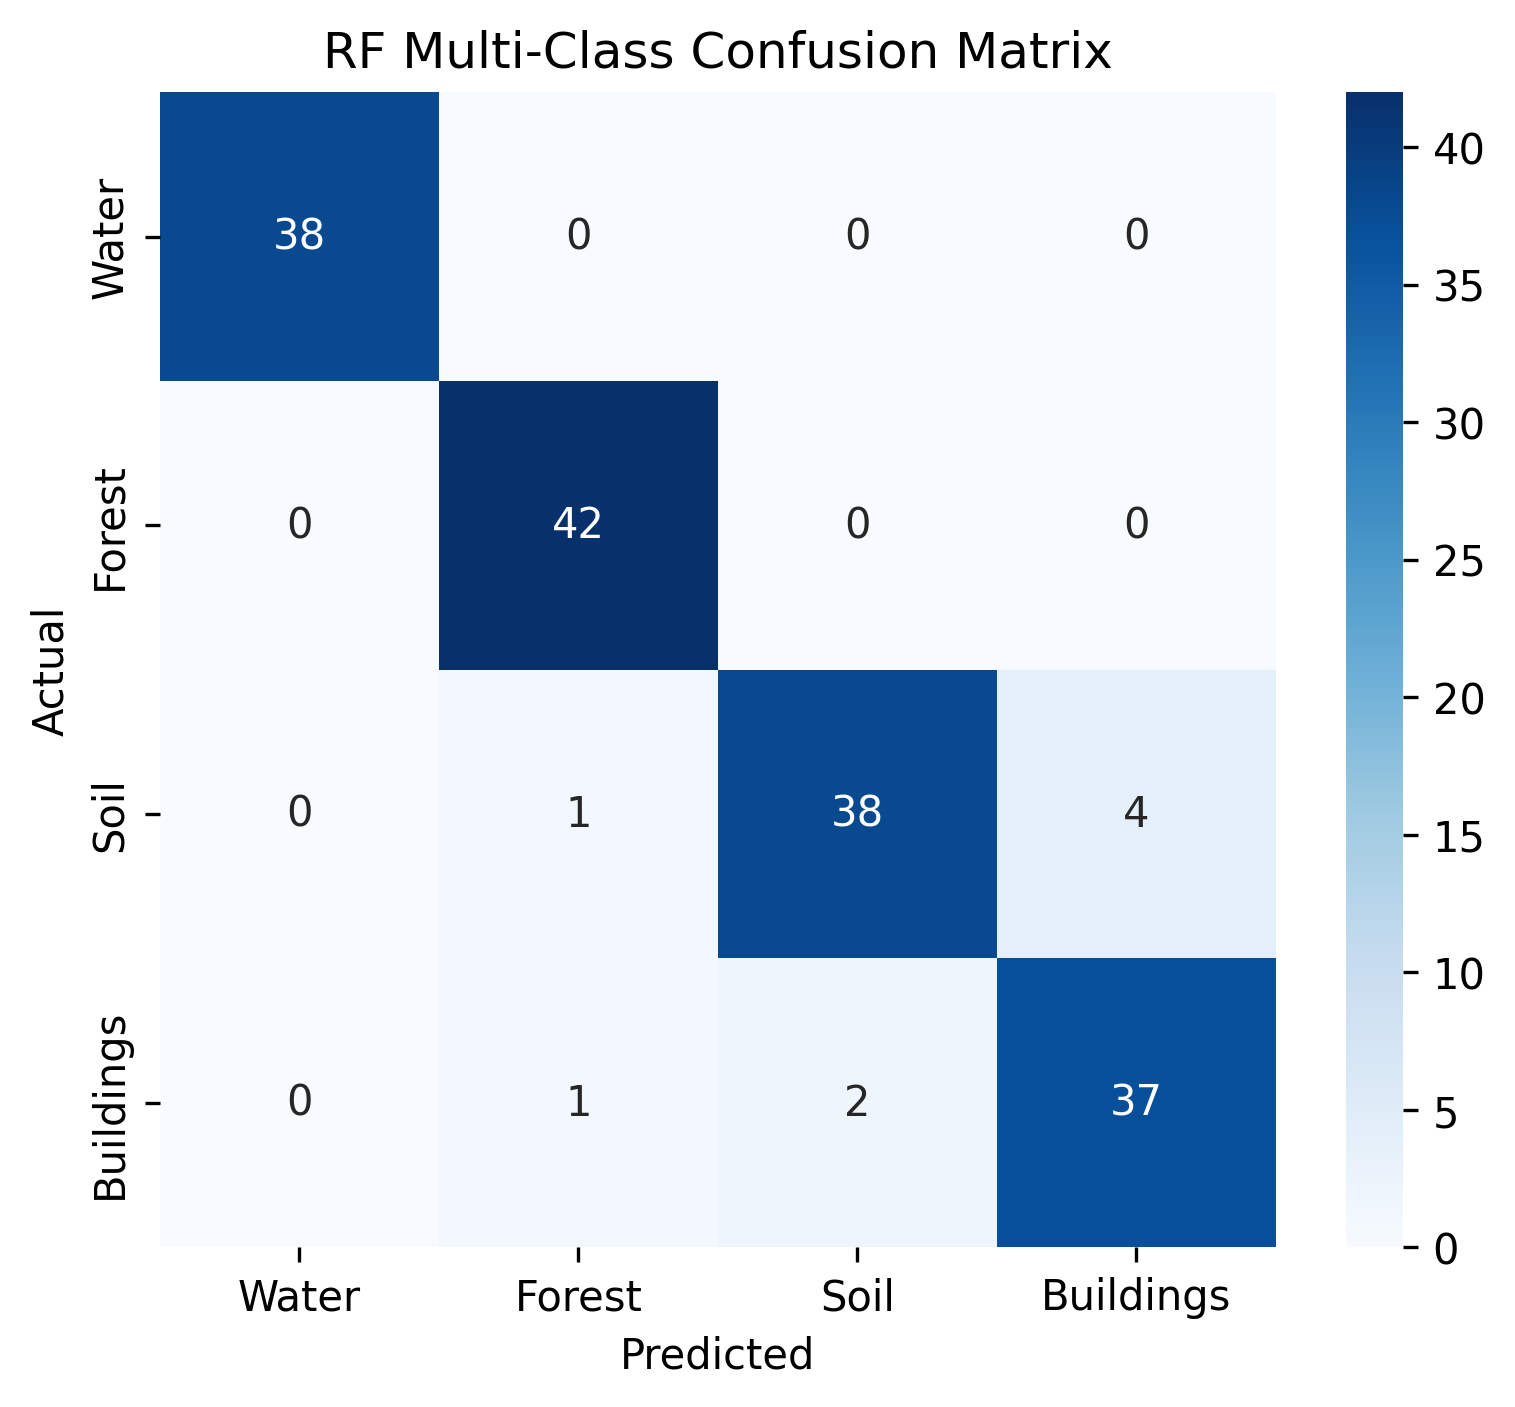
\includegraphics[width=\textwidth]{assets/multi_rf_cm.png}
        \caption{Random Forest}
    \end{subfigure}
    \hfill
    \begin{subfigure}[b]{0.45\columnwidth}
        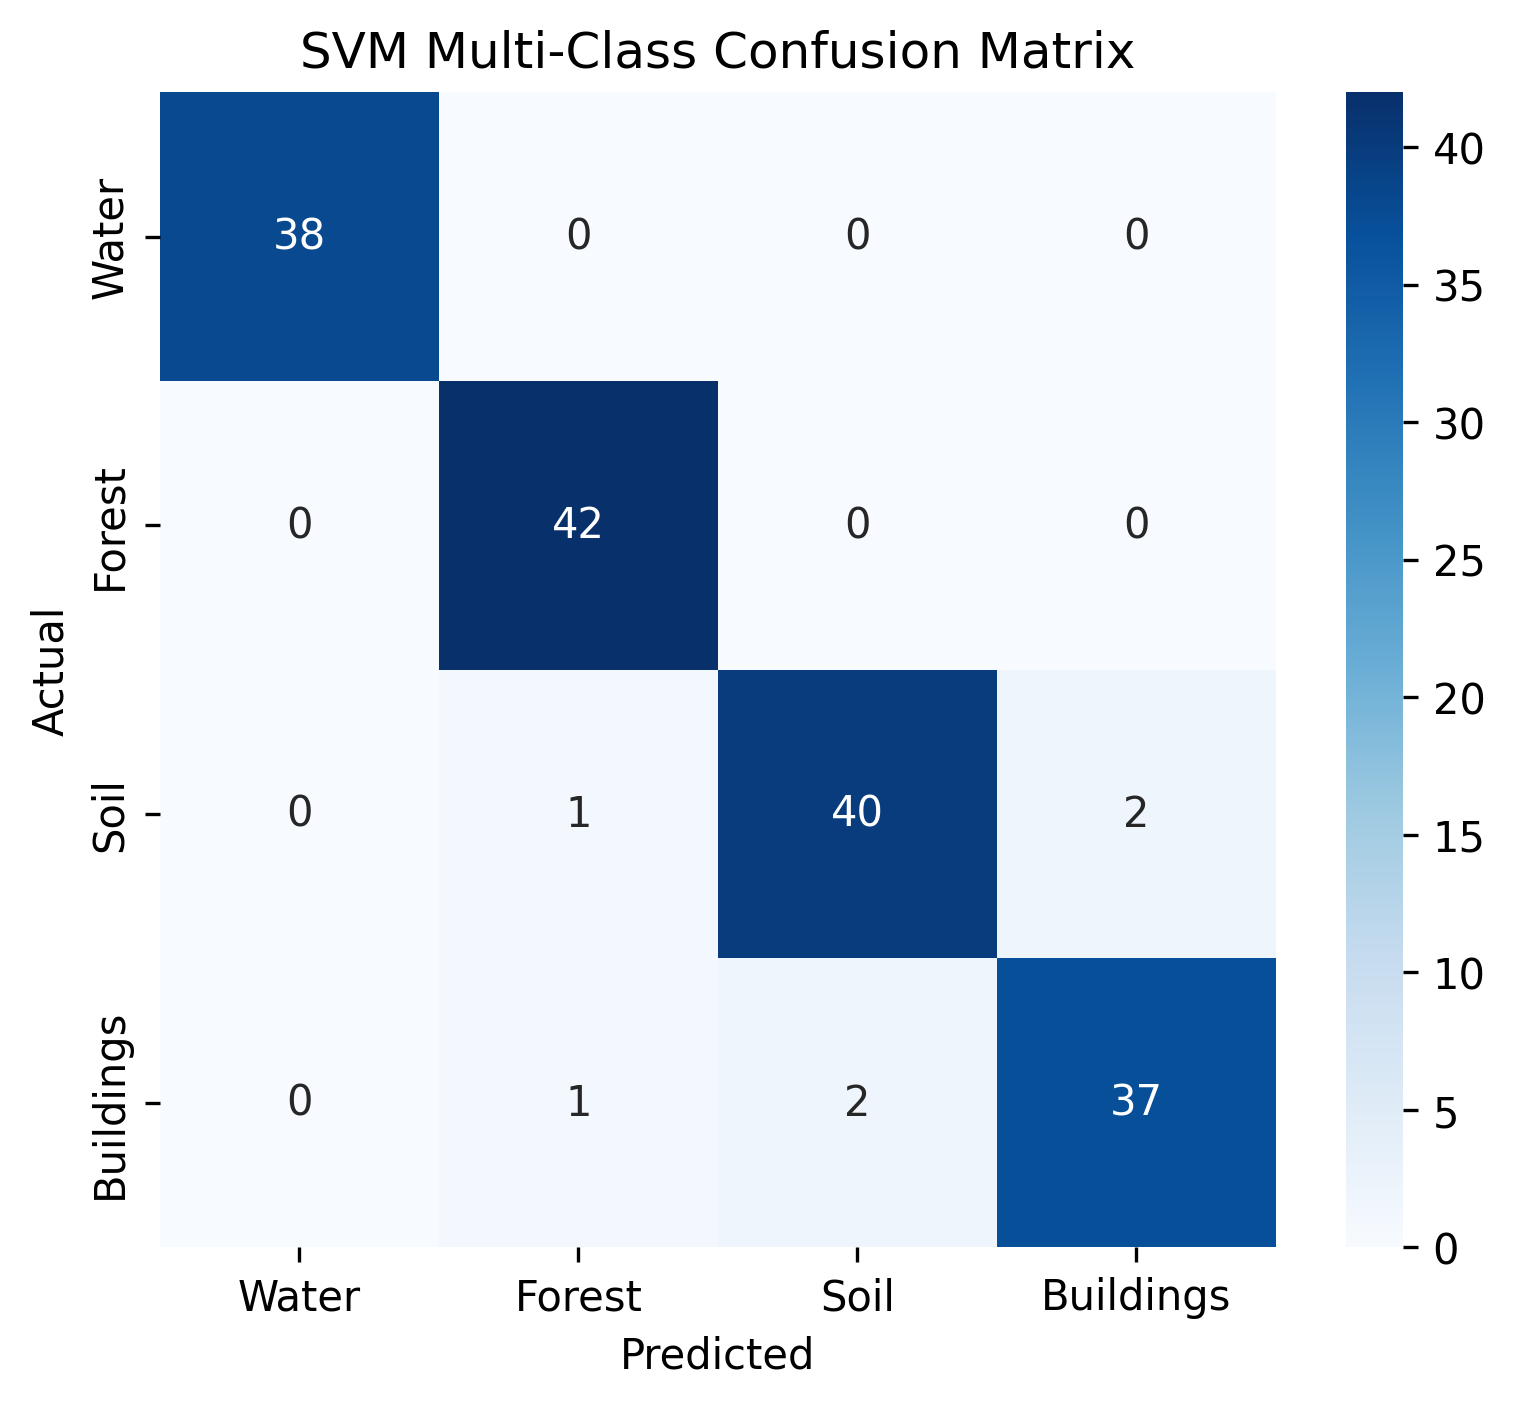
\includegraphics[width=\textwidth]{assets/multi_svm_cm.png}
        \caption{SVM (RBF)}
    \end{subfigure}
    \vskip\baselineskip
    \begin{subfigure}[b]{0.45\columnwidth}
        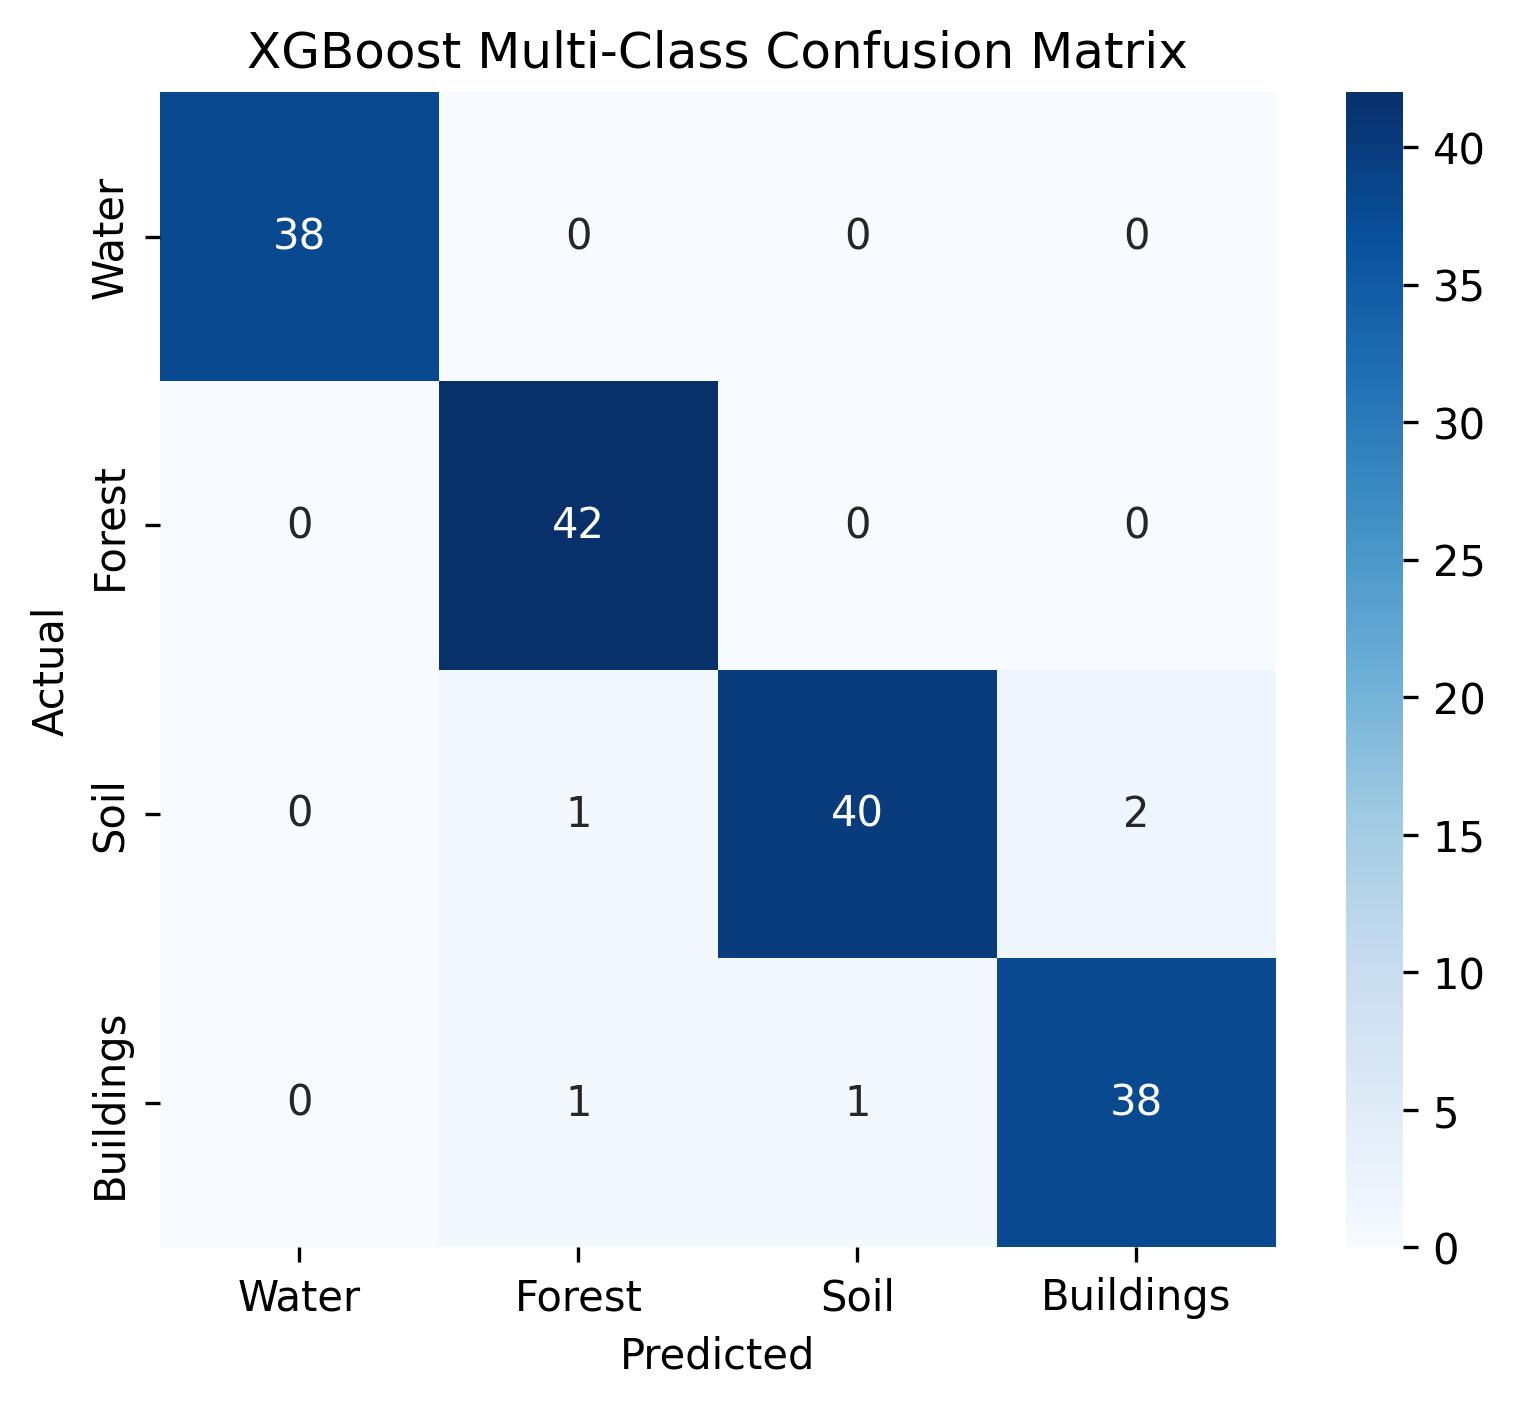
\includegraphics[width=\textwidth]{assets/multi_xgb_cm.png}
        \caption{XGBoost}
    \end{subfigure}
    \caption{Confusion matrices for the 4-class classification across the campus validation set.}
    \label{fig:multi_cm}
\end{figure}

%% ============================================================================
\section{Conclusion}
\label{sec:conclusion}

This study rigorously evaluated three supervised machine learning classifiers---Random Forest, Support Vector Machine (RBF kernel), and Gradient Boosted Trees (XGBoost)---for mapping Forest and Non-Forest regions via Sentinel-2 imagery. The principal findings are:

\begin{enumerate}
    \item \textbf{Model Generalization:} On a local subset extension out of the campus domain, SVM (RBF) yielded the highest external generalization accuracy (91.04\%), closely trailed by XGBoost (90.83\%). In deployment scenarios involving significant spatial variance, nonlinear boundary kernels outperform hierarchical variants.
    
    \item \textbf{District-Scale Transferability:} When deployed across the entire Jabalpur district ($\sim$5,211\,km$^2$) with 1,600 auto-generated test points, all three classifiers exceeded 97\% accuracy. SVM (RBF) again achieved the highest accuracy of 98.31\% ($\kappa = 0.966$), confirming that campus-trained models transfer effectively to district-scale landscapes within the same climatic zone when paired with appropriate imagery timing.
    
    \item \textbf{Optimal Hyperparameters:} Extensive localized searches verified that the architectures hit maximal empirical capacity when aggressively constrained, e.g., restricting Random Forest leaf partitions to \texttt{bagFraction=0.3} and pushing the SVM penalty to \texttt{Cost=100.0} combined with learning rates of \texttt{0.01} for boosting sequences.
    
    \item \textbf{Seasonal Phenomenological Imperatives:} Input data temporally dictates ceiling accuracy stronger than the underlying ML classification logic. The study statistically proves that \textbf{Winter (Jan-Feb) composites provide critical atmospheric separability} (90.0\% Accuracy) by waiting for undergrowth to physically dry up across the testing boundaries, completely bypassing the extreme misclassifications characteristic of the saturated Post-Monsoon period (70.4\% Accuracy). The strong Jabalpur results using Nov--Dec imagery further validate that the post-monsoon dry transition window is equally effective for large-area deployment.
\end{enumerate}

\subsection{Future Work}

\begin{itemize}
    \item \textbf{Multi-sensor arrays:} Injecting vertical-bouncing active radar methodologies such as Sentinel-1 SAR models into the input matrix to directly assess mathematical tree height, bypassing leaf-colour phenomenological challenges completely.
    \item \textbf{Multi-district scaling:} Extending the district-level validation framework to additional administrative regions across Madhya Pradesh to quantify cross-district transferability bounds.
\end{itemize}

%% ============================================================================
%% REFERENCES
%% ============================================================================
\begin{thebibliography}{99}

\bibitem{lu2007survey}
D.~Lu and Q.~Weng, ``A survey of image classification methods and techniques for improving classification performance,'' \textit{International Journal of Remote Sensing}, vol.~28, no.~5, pp.~823--870, 2007.

\bibitem{drusch2012sentinel}
M.~Drusch, U.~Del~Bello, S.~Carlier, \textit{et~al.}, ``Sentinel-2: ESA's optical high-resolution mission for GMES operational services,'' \textit{Remote Sensing of Environment}, vol.~120, pp.~25--36, 2012.

\bibitem{gorelick2017google}
N.~Gorelick, M.~Hancher, M.~Dixon, S.~Ilyushchenko, D.~Thau, and R.~Moore, ``Google Earth Engine: Planetary-scale geospatial analysis for everyone,'' \textit{Remote Sensing of Environment}, vol.~202, pp.~18--27, 2017.

\bibitem{rouse1974monitoring}
J.~W.~Rouse, R.~H.~Haas, J.~A.~Schell, and D.~W.~Deering, ``Monitoring vegetation systems in the Great Plains with ERTS,'' in \textit{Proc.\ Third Earth Resources Technology Satellite-1 Symposium}, pp.~309--317, 1974.

\bibitem{breiman2001random}
L.~Breiman, ``Random forests,'' \textit{Machine Learning}, vol.~45, no.~1, pp.~5--32, 2001.

\bibitem{cortes1995support}
C.~Cortes and V.~Vapnik, ``Support-vector networks,'' \textit{Machine Learning}, vol.~20, no.~3, pp.~273--297, 1995.

\bibitem{vapnik1998statistical}
V.~N.~Vapnik, \textit{Statistical Learning Theory}. New York: Wiley, 1998.

\bibitem{friedman2001greedy}
J.~H.~Friedman, ``Greedy function approximation: A gradient boosting machine,'' \textit{Annals of Statistics}, vol.~29, no.~5, pp.~1189--1232, 2001.

\bibitem{chen2016xgboost}
T.~Chen and C.~Guestrin, ``XGBoost: A scalable tree boosting system,'' in \textit{Proc.\ 22nd ACM SIGKDD International Conference on Knowledge Discovery and Data Mining}, pp.~785--794, 2016.

\end{thebibliography}

\end{document}
